\documentclass[11pt]{article}
%Gummi|061|=)
\usepackage[italian]{babel}
\usepackage[utf8x]{inputenc}
\usepackage{hyperref}
\usepackage{graphicx}
\usepackage{amsmath}
\usepackage{frontespizio}

\DeclareMathOperator{\Tr}{Tr}
\DeclareMathOperator{\Exp}{exp}
\DeclareMathOperator{\Log}{log}
\DeclareMathOperator{\Det}{det}

\title{Tecniche combinatorie nel Modello di Ising bidimensionale}
\author{Alberto Botto Poala\\
Relatore Prof. Marco Billò}
\date{14.04.14}
\begin{document}
\begin{titlepage}
\begin{center}

% Upper part of the page. The '~' is needed because \\
% only works if a paragraph has started.

\includegraphics[width=0.23\textwidth]{unito}~\\[1cm]


\textsc{\LARGE università degli studi di torino}\\[1.8cm]

\textsc{\Large Tesi di Laurea Triennale}\\[0.5cm]

% Title

{ \huge \bfseries Tecniche combinatorie nel Modello di Ising bidimensionale \\[0.5cm] }



% Author and supervisor
\begin{minipage}{0.4\textwidth}
\begin{flushleft} \large
\emph{Candidato}\\
Alberto \textsc{Botto Poala}
\end{flushleft}
\end{minipage}
\begin{minipage}{0.4\textwidth}
\begin{flushright} \large
\emph{Relatore} \\
Prof. Marco \textsc{Billò}
\end{flushright}
\end{minipage}

\vfill

% Bottom of the page
{14.04.14}

\end{center}
\end{titlepage}


\maketitle
\section{Sviluppo ad alte temperature}
\subsection{Il reticolo e l'Hamiltoniana}

Consideriamo un reticolo quadrato $L \times L$ periodico, con \emph{N} segmenti orizzontali e \emph{N} segmenti verticali congiungenti i suoi $N$ siti. Queste particolari connessioni, che coinvolgono solo i primi vicini, saranno d'ora in avanti chiamate \emph{link}. Si veda a titolo di esempio la figura \ref{reticolo3}.
\begin{figure}[h]
\centering
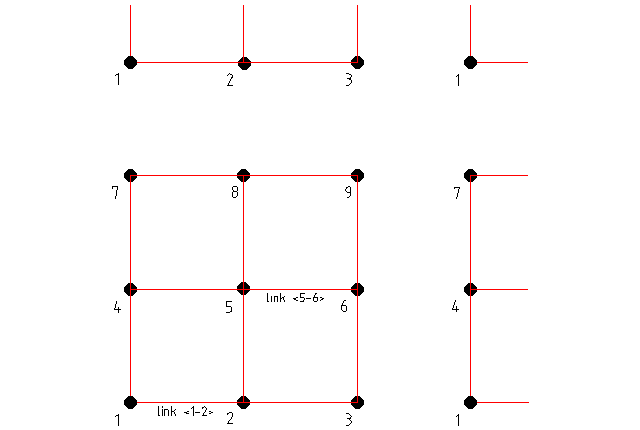
\includegraphics[width=0.86\columnwidth]{ret33}
\caption{Esempio di reticolo quadrato periodico $3 \times 3$ }
\label{reticolo3}
\end{figure}
\\Consideriamo due costanti di accoppiamento $J$ e $J'$ rispettivamente per i link orizzontali e verticali. La funzione di partizione è dunque
\begin{equation} \label{z}
Z_N=\sum_\sigma \exp \left[ K\sum_{(i,j)}\sigma_i\sigma_j+K'\sum_{(i,k)}\sigma_i\sigma_k \right]
\end{equation}
dove $(i,j)$ sono i link orizzontali, $(i,k)$ quelli verticali, mentre $K=\beta J$ e $K'=\beta J'$. Le variabili di spin $\sigma_i$ assumono i due valori $\pm1$.\\
Tramite l'identità
$$\exp[x\sigma_i\sigma_j]=\cosh{x}(1+\sigma_i\sigma_j\tanh{x})$$
si può riscrivere $Z_N$ come
\begin{equation}\label{z2}
Z_N=(\cosh{K}\cosh{K'})^N\sum_{\sigma}\left(\prod_{(i,j)}(1+v\sigma_i\sigma_j)\prod_{(i,k)}(1+w\sigma_i\sigma_k)\right) 
\end{equation}
dove $v=\tanh{K}$ e $w=\tanh{K'}$, sempre $\le1 \ \forall T $. Inoltre per $T\to\infty$ $v$ e $w$ tendono a $0$, e ciò ne giustificherà uno sviluppo in serie.
\subsection{Lo sviluppo in serie}
L'argomento tra parentesi tonde nell'equazione $\ref{z2}$, risultato del prodotto delle due produttorie, è formato da $2^{2N}$ termini: ogni produttoria è composta da $N$ termini (i link orizzontali o verticali) nella forma $(1+v\sigma_i\sigma_j)$ o $(1+w\sigma_i\sigma_k)$, una volta moltiplicati otteniamo ovviamente un prodotto di $2N$ termini nella stessa forma. Esplicitando il prodotto dei binomi tra parentesi si ottengono i $2^{2N}$ termini cercati, i primi sono:
$$
(1+v\sigma_{1}\sigma_{2})(1+v\sigma_{2}\sigma_{3})...(1+v\sigma_{j}\sigma_{j+1})...(1+w\sigma_{1}\sigma_{2})...(1+v\sigma_{k}\sigma_{k+1})=
$$
$$
1+v\sigma_{1}\sigma_{2}+v\sigma_{2}\sigma_{3}+...+v\sigma_{j}\sigma_{j+1}+...+w\sigma_{1}\sigma_{2}+...+w\sigma_{k}\sigma_{k+1}+...
$$
per passare via via a combinazioni più complesse, la cui forma generica è
\begin{equation}\label{geomest}
(v\sigma_{\alpha_1}\sigma_{\beta_1})\times... \times (v\sigma_{\alpha_r}\sigma_{\beta_r})\times (w\sigma_{\gamma_1}\sigma_{\delta_1}) \times... \times (w\sigma_{\gamma_s}\sigma_{\delta_s})
\end{equation}
a seconda di quali elementi si stiano selezionando all'interno del prodotto. I valori estremi che può assumere l'equazione $\ref{geomest}$ sono $1$ (se $r=s=0$) e $(vw)^M\sigma_1^4\sigma_2^4\times...\times\sigma_M^4$ (se $r=s=N$). Di sicuro vale $r,s \le N$. \\
 A questo punto possiamo prendere un generico elemento nella forma dell'espresione \ref{geomest} e, per ogni link orizzontale $(v\sigma_{\alpha_i}\sigma_{\beta_i})$ che trovo, lo evidenzio sul reticolo. Stesso procedimento per i link verticali.\\
 Se ad esempio dei $2^{2N}$ termini scegliamo
 \begin{equation}\label{esempioprod}
 (v\sigma_{5}\sigma_{6})(v\sigma_{6}\sigma_{7})(v\sigma_{11}\sigma_{12})(w\sigma_{1}\sigma_{5})(w\sigma_{10}\sigma_{14})
 \end{equation}
 otteniamo la figura \ref{confgraf} di sinistra. \\Un'altra possibile combinazione, di un tipo che in seguito scopriremo essere molto interessante, potrebbe essere
\begin{equation}\label{esempioprodchiuso}
(v\sigma_{1}\sigma_{2})(v\sigma_{5}\sigma_{6})(v\sigma_{6}\sigma_{7})(v\sigma_{10}\sigma_{11})(w\sigma_{1}\sigma_{5})(w\sigma_{2}\sigma_{6})(w\sigma_{6}\sigma_{10})(w\sigma_{7}\sigma_{11})
\end{equation}
a cui corrisponde la configurazione grafica destra in figura \ref{confgraf}.
\begin{figure}
\centering
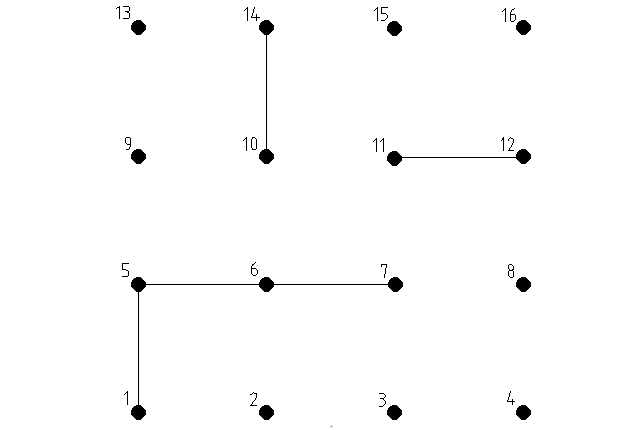
\includegraphics[width=0.47\columnwidth]{sat21}\quad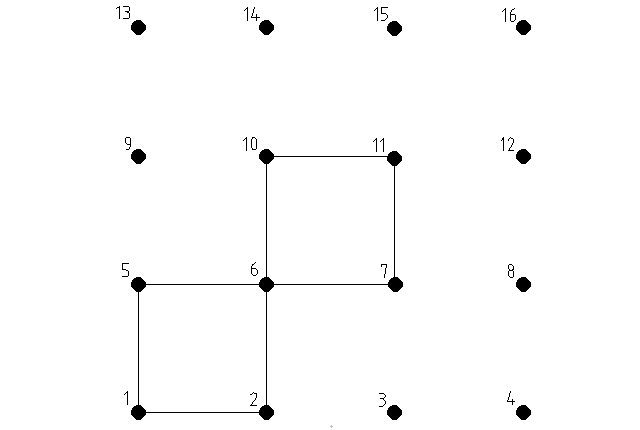
\includegraphics[width=0.47\columnwidth]{sat22}
\caption{configurazioni grafiche sul reticolo rispettivamente dell'equazione \ref{esempioprod} e \ref{esempioprodchiuso} }
\label{confgraf}
\end{figure}

 Abbiamo ottenuto un risultato importante, in quanto siamo riusciti ad  assegnare univocamente ad ogni elemento della sommatoria (un oggetto analitico) una configurazione grafica sul reticolo (un oggetto geometrico) e viceversa.
 Ora è anche chiaro perché avevamo introdotto due diverse costanti di accoppiamento $J$ e $J'$.\\
 Possiamo riscrivere questa quantità in maniera più compatta come
\begin{equation}\label{geomcom}
v^rw^s\sigma_1^{n_1}\sigma_2^{n_2}\sigma_3^{n_3}...
\end{equation}
dove $r$ è il numero di link orizzontali accesi, $s$ quelli verticali, e gli $n_i$ il numero di link che partono o finiscono nel sito $i$-esimo. Il prezzo da pagare è che diventa molto più complicato (anche se a rigor di logica sempre possibile) capire come disegnare il grafico associato, in quanto non sappiamo più se un generico $\sigma_{i}$ fosse associato ad un $v$ o un $w$. Sottolineiamo però che questa non è una perdita di informazioni, diventa solo più difficile reperirle.
\subsection{Simmetria della funzione di partizione}
A questo punto non dobbiamo dimenticarci che i termini discussi fin'ora erano nell'equazione \ref{z2} argomento di una sommatoria  estesa a tutte le configurazioni possibili degli spin sul reticolo, ovvero erano sommati al variare di tutte le possibili combinazioni di valori delle variabili $\sigma_i=\pm1$. Questo implica che se uno o più esponenti $n_i$ fossero dispari, il termine a cui appartengono non sopravvivrebbe nella sommatoria, in quanto verrebbe eliminato dal suo opposto. In altre parole stiamo dicendo che sopravvivono solo le espressioni \ $\ref{geomcom}$ \  simmetriche nelle variabili $\sigma_i$. \\
 L'interpretazione geometrica è che le configurazioni grafiche devono essere chiuse: non sopravvivono quelle che partono da un punto e arrivano in un altro, perché queste avrebbero $n_i=1$ (o $3$ se ripassa sul punto di partenza lungo il tragitto). Notiamo che è possibile che una configurazione grafica sia formata da più poligonali chiuse disgiunte, nel caso più semplice due quadrati, che però non possono avere un lato in comune. A tal proposito nella figura \ref{confgraf} sopravvivrebbe solo la configurazione di destra. Il problema delle sovrapposizioni verrà affrontato nella soluzione proposta da Vdovichenko, che vedremo in seguito.\\
Appurato ciò possiamo semplificare ulteriormente la $\ref{geomcom}$ in
\begin{equation}\label{eq:test}
v^rw^s
\end{equation} 
e ne avremo $2^N$ per ogni valore di \emph{r} e \emph{s}.\\
Riscriviamo quindi l'equazione \ref{z} come
\begin{equation}\label{z3}
Z_N=2^N(\cosh{K}\cosh{L})^M\sum_Pv^rw^s
\end{equation}
con $P$ insieme di tutte le poligonali chiuse che si possono accendere sul reticolo.\\
A parte dei coefficienti (dipendenti dalla temperatura), la funzione di partizione è univocamente determinata dalla quantità
\begin{equation}\label{serie}
\Phi(v,w)=\sum_Pv^rw^s
\end{equation}
Scrivere esplicitamente l'espressione \ref{serie} è molto complicato all'aumentare di $r$ e $s$, sia per quanto riguarda il calcolo della degenerazione, sia per il disegnare le configurazioni grafiche associate sul reticolo .\\ 
Se ci accontentiamo di sviluppare $\Phi$ ad alte temperature (quindi nelle variabili $v$ e $w$, che ricordiamo essere piccole ad alte $T$), otteniamo
\begin{equation}
\begin{split}
\Phi(v,w)=\sum_Pv^rw^s=\\
&=1+Nv^2w^2+Nv^2w^4+Nv^4w^2+
\\&+Nv^2w^6++Nv^6w^2+\frac{1}{2}N(N+5)v^4w^4...
\end{split}
\label{primiserie}
\end{equation}
Ogni termine ha associata, per quanto discusso prima, una ben definita configurazione grafica ed una degenerazione. Vediamone alcune:
\begin{itemize}
\item{ $1$ corrisponde a non aver tracciato nessun grafico} 
\item{$(vw)^2$ sono gli $N$ quadrati accendibili sul reticolo}
\item{ si presentano poi i rettangoli con perimetro di $6$ link con i lati maggiori verticali e orizzontali (anch'essi con degenerazione $N$). Idem per quelli da $8$}
\item{Il termine $v^4w^4$ porta le configurazioni grafiche di figura \ref{v4w4}. La degenerazione dei quadrati è ovviamente $N$, dei quadrati senza uno spigolo $4N$ ($N$ per ogni tipo). Quella della coppia di quadrati $N(N-5)/2$, in quanto dopo aver disegnato il primo ho $N-5$ posti dove mettere il secondo. Non posso infatti nè sovrapporlo nè metterlo con dei lati adiacenti. Sommando il questi tre termini ottengo $N(N+5)/2$}
\end{itemize} 
\begin{figure}[h]
\centering
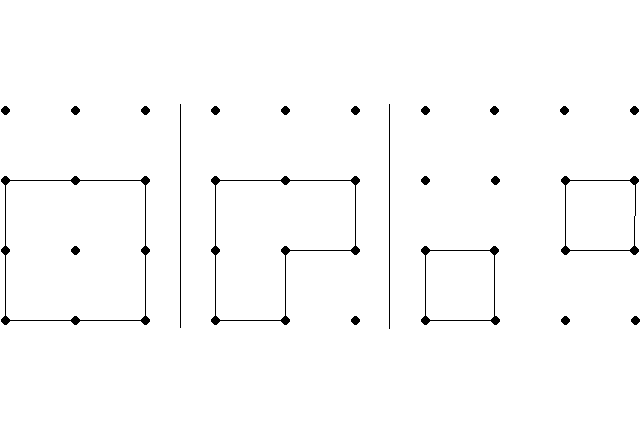
\includegraphics[width=0.73\columnwidth]{sat3}
\caption{configurazioni grafiche sul reticolo di $v^4w^4$ }
\label{v4w4}
\end{figure}



\section{Soluzione combinatoria di Vdovichenko}
\subsection{Configurazioni grafiche e cammini chiusi}

Vediamo ora la \emph{soluzione combinatoria di Vdovichenko}, che si prefigge l'obbiettivo di calcolare tutti i termini della serie. Stiamo quindi per affrontare una soluzione esatta e non una semplice approssimazione.\\
Nel capitolo precedente avevamo considerato due diverse costanti di accoppiamento $J$ e $J'$ con il solo scopo di separare le variabili $v$ e $w$, il ché ci ha permesso di comprendere meglio la configurazione grafica dei termini $v^rw^s$ sul reticolo.\\
D'ora in poi per semplicità considereremo $J=J'$ e quindi $v=w$: stiamo dicendo che i termini $v^4w^2$ e $v^2w^4$ nell'equazione \ref{primiserie} ora compaiono tutti come $v^6$, con degenerazione $2N$. \\
Definiamo inoltre come \emph{maglia} una sola poligonale chiusa, come \emph{grafico} l'unione di una o più maglie disgiunte.  \\
La funzione di partizione diventa dunque
\begin{equation}\label{enlib}
Z_N=2^N(1-v^2)^{-N}\Phi(v)
\end{equation}
con 
\begin{equation}
\Phi(v)= \sum_r g_r v^r
\end{equation}
dove $g_r$ è il numero di \emph{grafici} non necessariamente connessi con perimetro $r$ disegnabili sul reticolo. \\
Il primo obbiettivo di questo capitolo è scrivere questi grafici che avevamo evidenziato sul reticolo nello sviluppo ad alte temperature come dei \emph{cammini chiusi}.
Il problema sorge davanti alle ambiguità come quella in figura \ref{v1}, che può essere interpretata nei tre modi descritti.
\begin{figure}[h]
\centering
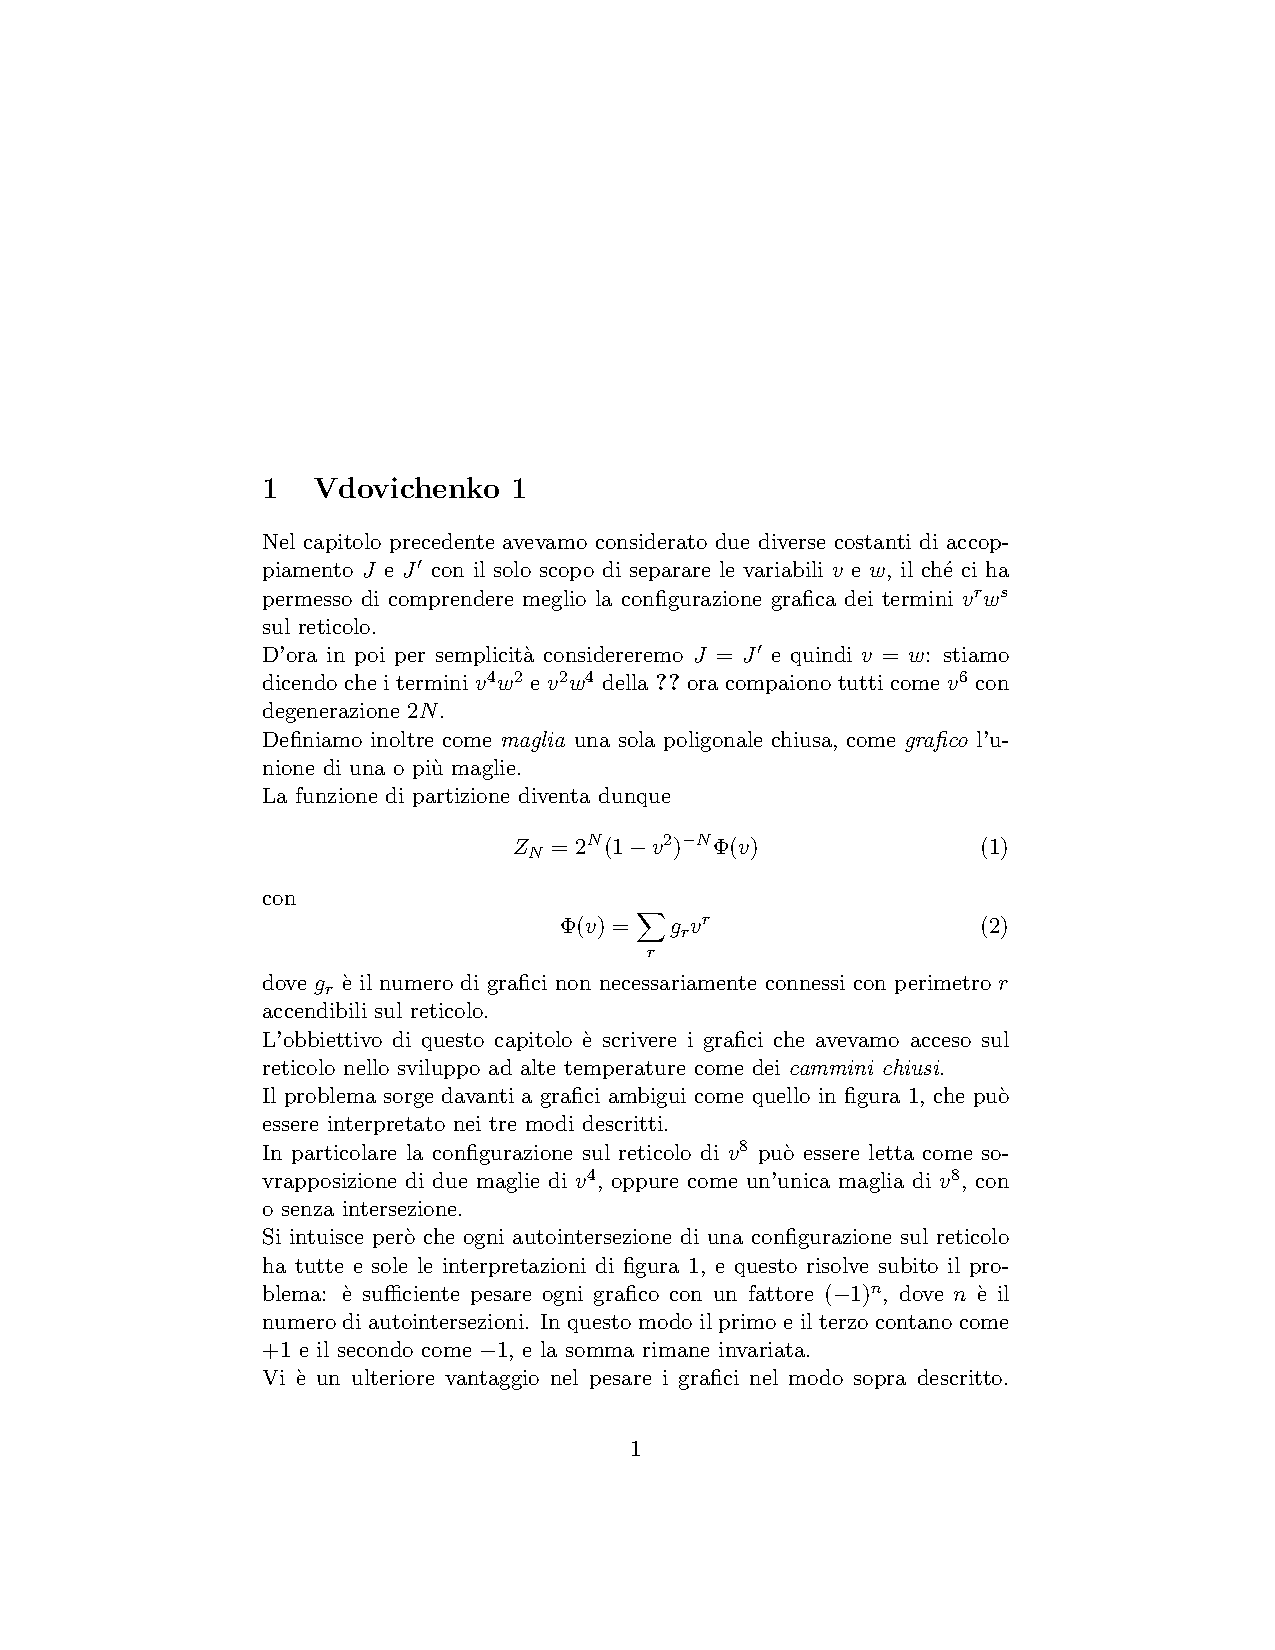
\includegraphics[width=0.5\columnwidth]{v1}
\caption{tre diversi grafici di $v^8$ con identica configurazione sul reticolo}
\label{v1}
\end{figure}
\\
In particolare la configurazione sul reticolo di $v^8$ può essere letta come sovrapposizione di due maglie di $v^4$, oppure come un'unica maglia di $v^8$, con o senza intersezione.\\
Si intuisce però che ogni autointersezione di una configurazione sul reticolo ha tutte e sole le interpretazioni di figura \ref{v1}, e questo risolve subito il problema: è sufficiente pesare ogni grafico con un fattore $(-1)^n$, dove $n$ è il numero di autointersezioni. In questo modo il primo e il terzo contano come $+1$ e il secondo come $-1$, e la somma rimane invariata.\\
Vi è un ulteriore vantaggio nel pesare i grafici nel modo sopra descritto. Come accennato precedentemente non è ammissibile come configurazione grafica sul reticolo di $v^8$ quella formata da due quadrati con un lato in comune: i due siti centrali avrebbero un numero dispari di ingressi/uscite, $\sigma_i$ sarebbe elevata al cubo, ed essendo antisimmetrica verrebbe, come già spiegato, eliminato. Nel caso però venissero contati, se pesati con il fattore $(-1)^n$ non darebbero comunque contributo, in quanto si eliminerebbero a vicenda. Si veda la figura \ref{v2} per capire come.
\begin{figure}[h]
\centering
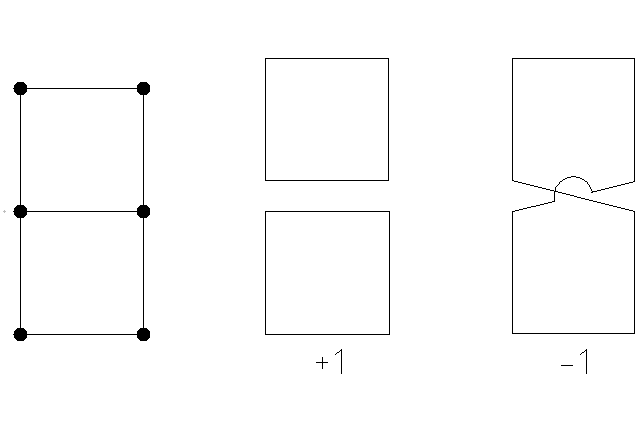
\includegraphics[width=0.45\columnwidth]{v2}
\caption{soluzione del problema della disparità nei siti $\sigma_i$}
\label{v2}
\end{figure}
\\
Bisogna quindi capire come determinare il numero di autointersezioni $n$ di una maglia. Il problema risiede nel fatto che questa è una proprietà globale, mentre noi lavoriamo in maniera locale, ovvero guardando spigolo dopo spigolo cosa succede. 
\subsection{Le autointersezioni e il Teorema di Gauss}
Il metodo che si utilizza è discendente del noto teorema di Gauss, che afferma che l'angolo spazzato dalla tangente su un cammino chiuso senza intersezioni è $2\pi$. Generalizzando si intuisce che questo angolo è $2\pi(k+1)$, con $k$ intero positivo o negativo che aumenta o diminuisce a seconda che le intersezioni avvengano in un verso oppure nell'altro, come spiegato intuitivamente in figura \ref{v3}.
\begin{figure}[h]
\centering
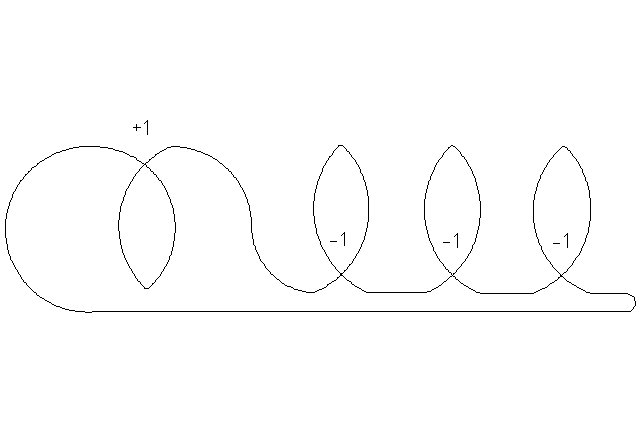
\includegraphics[width=0.65\columnwidth]{curva}
\caption{Generalizzazione del teorema di Gauss sull'angolo spazzato dalla tangente di una curva}
\label{v3}
\end{figure}
\\ La procedura da seguire è la seguente: ad ogni punto del cammino corrisponde un angolo di rotazione che può essere $\alpha=0,\pm\pi/2$. Se il percorso ruota di un angolo $\alpha$ gli attribuiamo una fase $e^{i\alpha/2}$ e per il teorema di Gauss, considerando i contributi di tutti i siti, acquisisce il valore $(-1)^{\nu+1}$, con $\nu$ somma delle intersezioni di una maglia, pesate del loro segno. Per un insieme di più maglie si ottiene $(-1)^{n+s}$ con $n=\sum\nu$ e $s$ numero di maglie. Ovviamente noi vorremmo ad esponente solo $n$ e non $s$, dopo vedremo come risolvere questo inconveniente.
\subsection{Grafici e maglie}
Chiamiamo ora con $f_r$ il numero di maglie di perimetro $r$ pesate nel modo sopra descritto. Il numero dei grafici composti da due maglie disgiunte pesate sarà
\begin{equation}\label{2maglia}
g_r^{(2)}=\frac{1}{2!}\sum_{r_1+r_2=r}f_{r_1}f_{r_2}
\end{equation}
dove ovviamente il $2!$ è necessario in quanto i grafici sono indistinguibili. Qui torna molto utile quanto discusso nella \ref{v2}, in quanto avremmo dovuto altrimenti fare un calcolo più complesso. Un generico grafico è composto da $s$ maglie, con $s$ variabile da $1$ a $+\infty$, quindi si scrive
\begin{equation} \label{phi}
\Phi(v)=\sum_{s=1}(-1)^s\frac{1}{s!}\sum_{r_1,r_2,...=0}^\infty v^{r_1+r_2+...r_s}f_{r_1}...f_{r_s}
\end{equation}
Il fattore $(-1)^s$ serve a compensare l'inconveniente lasciato in sospeso poche righe sopra, il fattore di simmetria $1/s!$ è la generalizzazione dell'$1/2!$ che appare nell'equazione \ref{2maglia}. Notiamo che gli esponenti $r_i$ assumono tutti i possibili valori da $1$ a $+\infty$ in tutte le possibili combinazioni, quindi anche $r=\sum_i r_i$. Possiamo quindi riorganizzare la sommatoria come
$$\sum_{r_1,r_2...=0}^\infty v^{r_1+r_2+...r_s}f_{r_1}...f_{r_s}=\left( \sum_{r=0}^\infty v^rf_r \right)^s$$
e sostituirla nell'equazione \ref{phi}, che riconosciamo subito essere uno sviluppo in serie di un esponenziale:
\begin{equation}\label{phi2}
 \Phi(v)= \exp \left[ - \sum_{r=0}^\infty v^r f_r \right]
\end{equation}
Resta da determinare la quantità $f_r$, cioè il numero di maglie chiuse.
\subsection{Parametrizzazione delle maglie}
Iniziamo indicizzando con $\mu=1,2,3,4$ gli spostamenti sul reticolo rispettivamente verso destra, in alto, sinistra, in basso.
L'informazione che daremo d'ora in avanti sarà sempre del tipo
$$ (coordinate \ del \ sito, \ direzione \ di \ ingresso \ nel \ sito)
$$
Decidiamo quindi di partire dal sito di coordinate $(i_0,j_0)$ con direzione \emph{di ingresso} in detto sito $\mu_0$. Notiamo che questa direzione non ha alcuna influenza sul cammino che stiamo per descrivere. Possiamo così introdurre la funzione $W_r(i,j,\mu)$ come il numero pesato di cammini che arrivano al punto $(i,j)$ con direzione $\mu$ dopo $r$ passi data o meno una condizione iniziale. Poniamo inoltre per comodità $\mu=\mu_0$, tanto come già detto $\mu_0$ non ha influenza sul cammino che stiamo per percorrere. Alcuni esempi dati $(i_0,j_0,\mu_0)=(0,0,1)$ sono (si veda la figura \ref{v6}):
\begin{itemize}
\item{$W_1(1,0,1)=1$ dobbiamo partire da $(0,0)$ diretti verso destra e dobbiamo arrivare in $(1,0)$ da sinistra. Ovviamente c'è solo una possibilità}
\item{$W_2(1,1,4)=e^{i\frac{\pi}{4}}$ anche qui una sola possibilità}
\item{$W_4(0,0,4)=2$}
\end{itemize}
\begin{figure}[h]
\centering
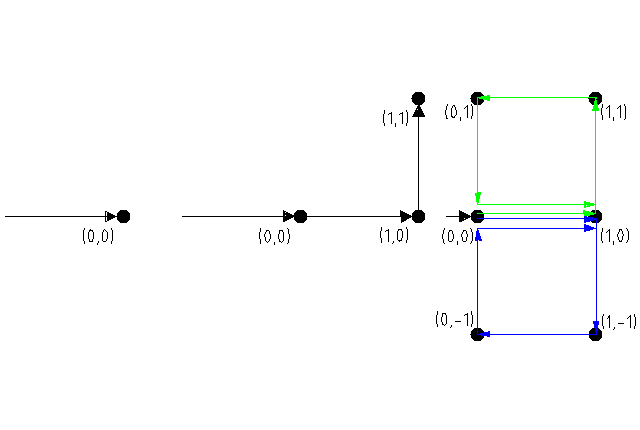
\includegraphics[width=0.8\columnwidth]{v6}
\caption{Esempi di camini sul reticolo}
\label{v6}
\end{figure}
 Questo siglifica che $W_r(i_0,j_0,\mu)$ indica il numero pesato di cammini che partono in $(i_0,j_0)$ dopo esserci arrivati con direzione $\mu_0=\mu$, e ci ritornano dopo $r$ passi nella direzione $\mu$. Possiamo quindi scrivere
 $$ f_r=\frac{1}{2r}\sum_{i_0,j_0,\mu}W_r(i_0,j_0,\mu)
 $$
dove il fattore $1/2r$ è necessario in quanto nella sommatoria un solo cammino è percorso nei due versi e partendo da ognuno dei suoi $r$ punti. 
La funzione $W_r(i,j,\mu)$ gode di proprietà ricorsive ben definite e facilmente intuibili, nella figura \ref{v7} rappresentiamo graficamente la prima.
\begin{equation}
\begin{aligned}
W_{r+1}(i,j,1) & = & W_r(i-1,j,1)+e^{-i\frac{\pi}{4}}W_r(i-1,j,2)+0+e^{i\frac{\pi}{4}}W_r(i-1,j,4) \\
W_{r+1}(i,j,2) & = & e^{i\frac{\pi}{4}}W_r(i,j-1,1)+W_r(i,j-1,2)+e^{-i\frac{\pi}{4}}W_r(i,j-1,3)+0 \\
W_{r+1}(i,j,3) & = & 0+e^{i\frac{\pi}{4}}W_r(i+1,j,2)+W_r(i+1,j,3)+e^{-i\frac{\pi}{4}}W_r(i+1,j,4) \\
W_{r+1}(i,j,4) & = & e^{-i\frac{\pi}{4}}W_r(i,j+1,2)+0+e^{i\frac{\pi}{4}}W_r(i,j+1,3)+W_r(i,j+1,4)
\end{aligned} 
\end{equation}
\begin{figure}[h]
\centering
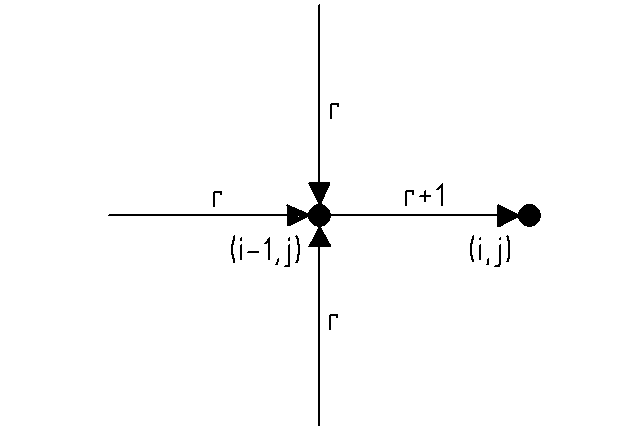
\includegraphics[width=0.7\columnwidth]{v7}
\caption{Rappresentazione grafica della prima equazione ricorsiva}
\label{v7}
\end{figure}

Come per ogni funzione ricorsiva, ad un certo punto arriviamo a chiederci quanto valga $W_0$. Questa funzione è perfettamente determinata dalle condizioni iniziali. \\
Esiste quindi un'applicazione lineare con matrice associata $\Lambda$ tale per cui
\begin{equation}\label{deflambda}
W_{r+1}(i,j,\mu)=\sum_{i',j',\mu'}\Lambda(ij\mu|i'j'\mu')W_{r}(i',j',\mu')
\end{equation}
Notiamo che $\Lambda$ è funzione non solo degli indici direzionali $\mu$ e $\mu'$, che variano da 1 a 4, ma anche di quelli di posizione. Stiamo quindi parlando di una matrice di grandi dimensioni.\\
$\Lambda$ è l'oggetto che fa evolvere il sistema, ci dice quali cammini sono permessi e con quali fasi associate.\\
I suoi elementi di matrice sono il numero di modi di partire dal sito $(i_0,j_0)$ dopo esserci arrivati con direzione $\mu_0$ e di arrivare al sito $(i,j)$ con direzione $\mu$ dopo $r$ passi. Di conseguenza il generico elemento diagonale $\Lambda(i_0,j_0,\mu|I_0,j_0,\mu_0)$ altro non è che il numero di cammini che partono in $(i_0,j_0)$ e ci ritornano con direzione $\mu=\mu_0$. Notiamo che stiamo parlando di cammini chiusi.
Detto ciò intuiamo che la traccia di $\Lambda^r$
$$ \Tr{(\Lambda^r)}=\sum_{i_0,j_0,\mu} \Lambda^r(i_0,j_0,\mu|I_0,j_0,\mu_0)
$$ altro non è che il numero di cammini chiusi, a fissato $r$, che si possono percorrere sul reticolo. Questa quantità è legata al numero di maglie grazie alla relazione
\begin{equation}
f_r=\frac{1}{2r}\sum_{i_0,j_0,\mu} \Lambda^r(i_0,j_0,\mu|I_0,j_0,\mu_0)=\frac{1}{2r}\Tr{(\Lambda^r)}
\end{equation}
Come sappiamo la traccia è un invariante per cambio di base e, nell'ipotesi in cui siamo in grado di diagonalizzare $\Lambda$, possiamo scrivere
\begin{equation}\label{autovalori}
 f_r=\frac{1}{2r}\Tr{(\Lambda^r)}=\frac{1}{2r}\sum_a \lambda_a^r
\end{equation}
dove ovviamente $\lambda_a$ sono gli autovalori di $\Lambda$. Sostituendo questa espressione nell'equazione \ref{phi2} troviamo
\begin{equation}\label{prod}
\Phi(v)= \Exp \left [ -\frac{1}{2}\sum_i\sum_{r=1}^\infty\frac{1}{r}v^r\lambda_i^r \right ] = \Exp \left [ \frac{1}{2} \sum_i \Log (1-v\lambda_i) \right]= \prod_i \sqrt{1-v\lambda_i}
\end{equation}
nella quale le uniche incognite da determinare sono gli autovalori.\\
La strada più semplice per diagonalizzare $\Lambda$ è trasformarla secondo Fourier rispetto alle coordinate sul reticolo. Partiamo dalla trasformata secondo Fourier della quantità $W_r$ definita come segue:
\begin{equation}\label{trasformata}
W_r(p,q,\mu)=\sum_{k,l=0}^L e^{\frac{-2\pi i}{L}(pk+ql)}W_r(k,l,\mu)
\end{equation} 
dove $p$ e $q$ assumono i valori da $1$ a $L$.\\
Riconsideriamo poi l'espressione dell'equazione ricorsiva \ref{deflambda} dopo tale trasformazione.
Con semplici calcoli, assume la seguente forma:
$$
\left( \begin{array}{c}
W_{r+1}(p,q,1) \\
W_{r+1}(p,q,2)  \\
W_{r+1}(p,q,3) \\
W_{r+1}(p,q,4) \end{array} \right)=
\left( \begin{array}{cccc}
\epsilon^{-p} & \alpha^{-1}\epsilon^{-p} & 0 & \alpha\epsilon^{-p} \\
\alpha\epsilon^{-q} & \epsilon^{-q} & \alpha^{-1}\epsilon^{-q} & 0\\
0 & \alpha\epsilon^p & \epsilon^p & \alpha^{-1}\epsilon^p \\
\alpha^{-1}\epsilon^q & 0 &\alpha\epsilon^q & \epsilon^q \end{array} \right)
\left( \begin{array}{c}
W_{r}(p,q,1) \\
W_{r}(p,q,2)  \\
W_{r}(p,q,3) \\
W_{r}(p,q,4) \end{array} \right)
$$
dove $\epsilon=e^{\frac{2\pi i}{L}}$.\\
Notiamo che sia a destra che a sinistra le variabili sono $(p,q)$; confrontando con l'espressione \ref{deflambda} notiamo che la trasformata della matrice $\Lambda$ è diagonale negli indici $p$ e $q$
$$\Lambda(p,q,\mu | p',q',\mu')= \left(  \begin{array}{cccc}
\epsilon^{-p} & \alpha^{-1}\epsilon^{-p} & 0 & \alpha\epsilon^{-p} \\
\alpha\epsilon^{-q} & \epsilon^{-q} & \alpha^{-1}\epsilon^{-q} & 0\\
0 & \alpha\epsilon^p & \epsilon^p & \alpha^{-1}\epsilon^p \\
\alpha^{-1}\epsilon^q & 0 &\alpha\epsilon^q & \epsilon^q \end{array} \right)\delta_{pp'}\delta_{qq'}
$$
Se riprendiamo ora l'equazione \ref{prod} possiamo scrivere la produttoria tramite la matrice $\Lambda$ non diagonalizzata come
$$
\prod_i1-v\lambda_i=\Det(\textbf{1}-v\Lambda)=(1+v^2)^2-2v(1-v^2) \left( \cos{\frac{2\pi p}{L}}+\cos{\frac{2\pi q}{L}} \right)
$$
Sostituendo tale risultato nell'espressione \ref{enlib} della funzione di partizione otteniamo
$$
Z_N=2^N(1-v^2)^{-N}\prod_{p,q=0}^L \left[ (1+v^2)-2v(1-v^2) \left( \cos{\frac{2\pi p}{L}}+\cos{\frac{2\pi q}{L}} \right) \right]^{\frac{1}{2}}
$$ 
\subsection{L'energia libera}
L'energia libera è calcolata dunque come
\begin{equation}
\begin{split}
\frac{-F(T)}{kT}=\Log(Z_N)=\\
&=N\Log(2)-N\Log(1-v^2)+\\
&+\frac{1}{2} \sum_{p,q=0}^L\Log\left[ (1+v^2)-2v(1-v^2) \left( \cos{\frac{2\pi p}{L}}+\cos{\frac{2\pi q}{L}} \right) \right]
\end{split}
\end{equation}
Nel limite termodinamico per cui $L\to+\infty$ la somma si trasforma in un integrale definito
\begin{equation}
\begin{split}
\frac{-F(T)}{kT}=\\
&=N\Log(2)-N\Log(1-v^2)+
\\&+\frac{N}{2(2\pi)^2}\int_0^{2\pi}\int_0^{2\pi} d\omega_1 d\omega_2 \Log\left[ (1+v^2)-2v(1-v^2) \left( \cos{\omega_1}+\cos{\omega_2} \right) \right]
\end{split}
\end{equation}
Notiamo che la $F(T)$ ottenuta è estensiva, in quanto direttamente proporzionale al numero di siti del reticolo $N$.\\
Nota $F(T)$ si può derivare la termodinamica.


\end{document}

